\documentclass{article}
\usepackage[utf8]{inputenc}

% Essential packages for article format
\usepackage{amsmath, amssymb, amsfonts}
\usepackage{bm}
\usepackage{graphicx}
\usepackage{xcolor}
\usepackage{tcolorbox}
\usepackage[bookmarks=false]{hyperref}
\usepackage{url}
\usepackage{booktabs}
\usepackage{array}
\usepackage{multirow}
\usepackage{enumitem}
\usepackage{tikz}
\usetikzlibrary{arrows.meta, positioning, shapes.geometric}

% Additional packages for a nice tutorial format
\usepackage[margin=1in]{geometry}
\usepackage{fancyhdr}
\usepackage{titlesec}

% Header and footer setup
\pagestyle{fancy}
\fancyhf{}
\rhead{Tutorial: Cross-Validation}
\lhead{ES335 - Machine Learning}
\rfoot{Page \thepage}

% Title formatting
\titleformat{\section}{\Large\bfseries\color{blue!75!black}}{\thesection}{1em}{}
\titleformat{\subsection}{\large\bfseries\color{blue!60!black}}{\thesubsection}{1em}{}

% Load conventions after math packages
\usepackage{../../shared/styles/conventions}

% Define counters for examples and exercises
\newcounter{example}
\setcounter{example}{0}
\newcounter{exercise}
\setcounter{exercise}{0}

\title{\textbf{Tutorial: Cross-Validation} \\ \textit{Robust Model Evaluation and Selection}}
\author{ES335 - Machine Learning \\ IIT Gandhinagar}
\date{\today}

\begin{document}

\maketitle

\begin{abstract}
Cross-validation is a fundamental technique for evaluating machine learning models and selecting optimal hyperparameters. This tutorial covers the theory, implementation, and best practices of various cross-validation methods, from basic k-fold to advanced techniques for time series and grouped data. Learn how to avoid common pitfalls and obtain reliable performance estimates for your models.
\end{abstract}

\tableofcontents
\newpage

\section{Introduction: The Model Evaluation Challenge}

Imagine you've built a spam email classifier that achieves 99\% accuracy on your training data. Is this a good model? Without proper evaluation, you can't tell if your model is genuinely good or just memorizing the training data.

\textbf{The Core Problem}: How do we get reliable estimates of model performance?

\begin{center}
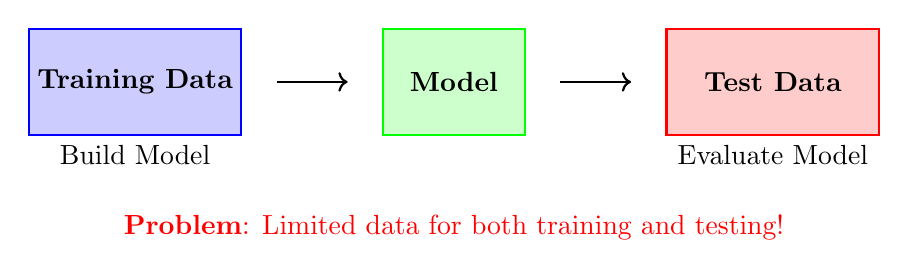
\begin{tikzpicture}[scale=0.9]
    % Training data
    \draw[thick, blue, fill=blue!20] (0,0) rectangle (3,1.5);
    \node at (1.5,0.75) {\textbf{Training Data}};
    \node[below] at (1.5,0) {Build Model};
    
    % Arrow
    \draw[->, thick] (3.5,0.75) -- (4.5,0.75);
    
    % Model
    \draw[thick, green, fill=green!20] (5,0) rectangle (7,1.5);
    \node at (6,0.75) {\textbf{Model}};
    
    % Arrow
    \draw[->, thick] (7.5,0.75) -- (8.5,0.75);
    
    % Test data
    \draw[thick, red, fill=red!20] (9,0) rectangle (12,1.5);
    \node at (10.5,0.75) {\textbf{Test Data}};
    \node[below] at (10.5,0) {Evaluate Model};
    
    % Problem illustration
    \node[red, below] at (6,-1) {\textbf{Problem}: Limited data for both training and testing!};
\end{tikzpicture}
\end{center}

\textbf{Simple Train/Test Split Limitations}:
\begin{itemize}
    \item Wastes data (typically 20-30\% held out)
    \item Performance depends on particular split
    \item No systematic hyperparameter tuning
    \item High variance in performance estimates
\end{itemize}

\section{K-Fold Cross-Validation}

\subsection{The Basic Idea}

K-fold cross-validation solves the data limitation problem by using each data point for both training and testing, but never simultaneously.

\textbf{Algorithm}:
\begin{enumerate}
    \item Divide dataset into $k$ equal-sized folds
    \item For each fold $i = 1, \ldots, k$:
    \begin{itemize}
        \item Use fold $i$ as test set
        \item Use remaining $k-1$ folds as training set
        \item Train model and evaluate on test fold
    \end{itemize}
    \item Average performance across all $k$ folds
\end{enumerate}

\begin{center}
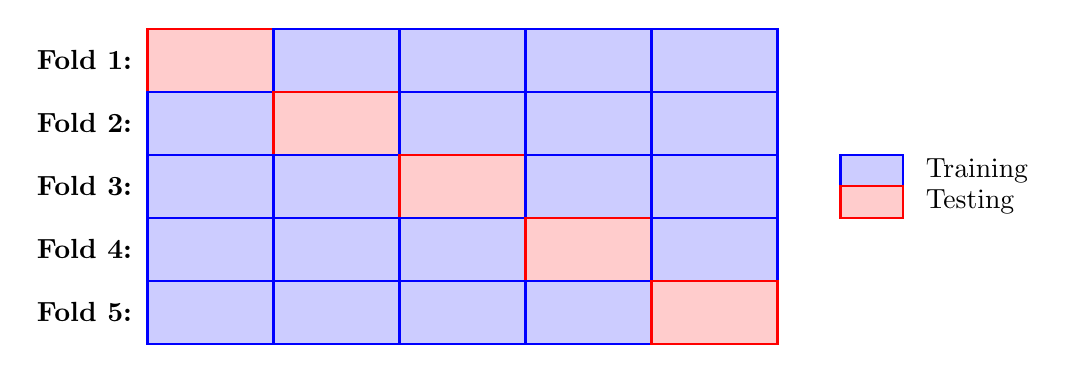
\begin{tikzpicture}[scale=0.8]
    % Fold 1
    \node at (-1,4) {\textbf{Fold 1:}};
    \draw[thick, red, fill=red!20] (0,3.5) rectangle (2,4.5);
    \draw[thick, blue, fill=blue!20] (2,3.5) rectangle (4,4.5);
    \draw[thick, blue, fill=blue!20] (4,3.5) rectangle (6,4.5);
    \draw[thick, blue, fill=blue!20] (6,3.5) rectangle (8,4.5);
    \draw[thick, blue, fill=blue!20] (8,3.5) rectangle (10,4.5);
    
    % Fold 2  
    \node at (-1,3) {\textbf{Fold 2:}};
    \draw[thick, blue, fill=blue!20] (0,2.5) rectangle (2,3.5);
    \draw[thick, red, fill=red!20] (2,2.5) rectangle (4,3.5);
    \draw[thick, blue, fill=blue!20] (4,2.5) rectangle (6,3.5);
    \draw[thick, blue, fill=blue!20] (6,2.5) rectangle (8,3.5);
    \draw[thick, blue, fill=blue!20] (8,2.5) rectangle (10,3.5);
    
    % Fold 3
    \node at (-1,2) {\textbf{Fold 3:}};
    \draw[thick, blue, fill=blue!20] (0,1.5) rectangle (2,2.5);
    \draw[thick, blue, fill=blue!20] (2,1.5) rectangle (4,2.5);
    \draw[thick, red, fill=red!20] (4,1.5) rectangle (6,2.5);
    \draw[thick, blue, fill=blue!20] (6,1.5) rectangle (8,2.5);
    \draw[thick, blue, fill=blue!20] (8,1.5) rectangle (10,2.5);
    
    % Fold 4
    \node at (-1,1) {\textbf{Fold 4:}};
    \draw[thick, blue, fill=blue!20] (0,0.5) rectangle (2,1.5);
    \draw[thick, blue, fill=blue!20] (2,0.5) rectangle (4,1.5);
    \draw[thick, blue, fill=blue!20] (4,0.5) rectangle (6,1.5);
    \draw[thick, red, fill=red!20] (6,0.5) rectangle (8,1.5);
    \draw[thick, blue, fill=blue!20] (8,0.5) rectangle (10,1.5);
    
    % Fold 5
    \node at (-1,0) {\textbf{Fold 5:}};
    \draw[thick, blue, fill=blue!20] (0,-0.5) rectangle (2,0.5);
    \draw[thick, blue, fill=blue!20] (2,-0.5) rectangle (4,0.5);
    \draw[thick, blue, fill=blue!20] (4,-0.5) rectangle (6,0.5);
    \draw[thick, blue, fill=blue!20] (6,-0.5) rectangle (8,0.5);
    \draw[thick, red, fill=red!20] (8,-0.5) rectangle (10,0.5);
    
    % Legend
    \draw[thick, blue, fill=blue!20] (11,2) rectangle (12,2.5);
    \node[right] at (12.2,2.25) {Training};
    \draw[thick, red, fill=red!20] (11,1.5) rectangle (12,2);
    \node[right] at (12.2,1.75) {Testing};
\end{tikzpicture}
\end{center}

\subsection{Mathematical Foundation}

Let $f^{(-i)}$ be the model trained on all data except fold $i$, and let $D_i$ be the test fold $i$.

\textbf{Cross-validation estimate}:
$$\text{CV}_k = \frac{1}{k} \sum_{i=1}^k L(f^{(-i)}, D_i)$$

where $L$ is the loss function (e.g., 0-1 loss for classification, MSE for regression).

\textbf{Standard error}:
$$\text{SE} = \sqrt{\frac{\sum_{i=1}^k (L_i - \text{CV}_k)^2}{k(k-1)}}$$

\begin{tcolorbox}[colback=blue!5!white,colframe=blue!75!black,title=Example \stepcounter{example}\#\theexample: 5-Fold CV Calculation]

Suppose you get these accuracy scores from 5-fold CV: [0.85, 0.82, 0.88, 0.86, 0.84]

\textbf{Mean accuracy}: $\mu = \frac{0.85 + 0.82 + 0.88 + 0.86 + 0.84}{5} = 0.85$

\textbf{Standard deviation}: $\sigma = \sqrt{\frac{(0.85-0.85)^2 + (0.82-0.85)^2 + \ldots}{5}} = 0.022$

\textbf{Report}: $85.0\% \pm 2.2\%$ accuracy

This means we're confident the true accuracy is between roughly 82.8\% and 87.2\%.
\end{tcolorbox}

\section{Cross-Validation Variants}

\subsection{Leave-One-Out Cross-Validation (LOOCV)}

Special case where $k = n$ (number of samples). Each fold contains exactly one sample.

\textbf{Advantages}:
\begin{itemize}
    \item Maximum use of training data ($n-1$ samples)
    \item Deterministic (no randomness in splits)
    \item Unbiased estimate of generalization error
\end{itemize}

\textbf{Disadvantages}:
\begin{itemize}
    \item Computationally expensive ($n$ model fits)
    \item High variance (each test set is tiny)
    \item Not suitable for model selection
\end{itemize}

\textbf{Mathematical property for linear models}:
$$\text{LOOCV} = \frac{1}{n} \sum_{i=1}^n \left(\frac{y_i - \hat{y}_i}{1 - h_{ii}}\right)^2$$

where $h_{ii}$ is the $i$-th diagonal element of the hat matrix. This allows LOOCV computation with a single model fit!

\subsection{Stratified Cross-Validation}

For classification problems, regular k-fold might create imbalanced folds. Stratified CV maintains class distribution in each fold.

\begin{tcolorbox}[colback=green!5!white,colframe=green!75!black,title=Example \stepcounter{example}\#\theexample: Why Stratification Matters]

\textbf{Dataset}: 1000 samples, 90\% negative (900), 10\% positive (100)

\textbf{Regular 5-fold}: Might create folds with 0-40 positive examples
\textbf{Stratified 5-fold}: Each fold has exactly 20 positive examples

Without stratification, some folds might have no positive examples, leading to misleading performance estimates!
\end{tcolorbox}

\textbf{Algorithm}:
\begin{enumerate}
    \item For each class, divide samples into $k$ groups
    \item Combine corresponding groups from each class to form folds
    \item Ensures each fold has approximately the same class distribution
\end{enumerate}

\subsection{Group Cross-Validation}

When samples are not independent (e.g., multiple measurements from same patient), regular CV can leak information.

\textbf{Examples of grouped data}:
\begin{itemize}
    \item Medical: Multiple visits per patient
    \item Finance: Multiple quarters per company  
    \item Time series: Multiple observations per entity
    \item Images: Multiple crops from same image
\end{itemize}

\textbf{Solution}: Ensure all samples from the same group are in the same fold.

\section{Time Series Cross-Validation}

Time series data violates the independence assumption of regular CV. We cannot use future data to predict the past!

\subsection{Forward Chaining (Walk-Forward Validation)}

\begin{center}
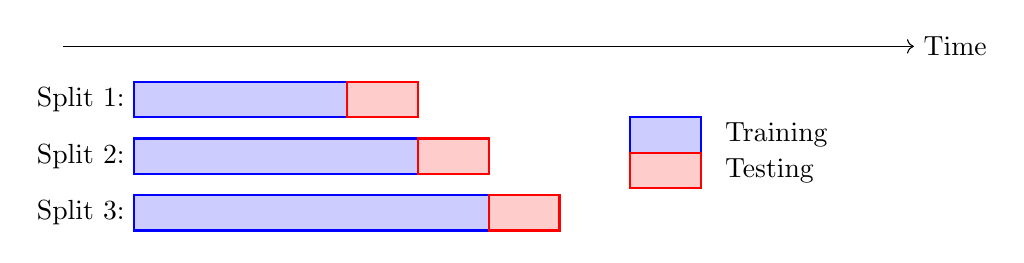
\begin{tikzpicture}[scale=0.9]
    % Timeline
    \draw[->] (0,3) -- (12,3) node[right] {Time};
    
    % Split 1
    \draw[thick, blue, fill=blue!20] (1,2) rectangle (4,2.5);
    \draw[thick, red, fill=red!20] (4,2) rectangle (5,2.5);
    \node[left] at (1,2.25) {Split 1:};
    
    % Split 2  
    \draw[thick, blue, fill=blue!20] (1,1.2) rectangle (5,1.7);
    \draw[thick, red, fill=red!20] (5,1.2) rectangle (6,1.7);
    \node[left] at (1,1.45) {Split 2:};
    
    % Split 3
    \draw[thick, blue, fill=blue!20] (1,0.4) rectangle (6,0.9);
    \draw[thick, red, fill=red!20] (6,0.4) rectangle (7,0.9);
    \node[left] at (1,0.65) {Split 3:};
    
    % Legend
    \draw[thick, blue, fill=blue!20] (8,1.5) rectangle (9,2);
    \node[right] at (9.2,1.75) {Training};
    \draw[thick, red, fill=red!20] (8,1) rectangle (9,1.5);
    \node[right] at (9.2,1.25) {Testing};
\end{tikzpicture}
\end{center}

\textbf{Key principles}:
\begin{itemize}
    \item Always train on past data, test on future data
    \item Training window can be expanding or fixed-size
    \item Gap between train/test to account for lag
\end{itemize}

\subsection{Blocked Cross-Validation}

For time series with seasonal patterns, create blocks that respect temporal structure:

\begin{center}
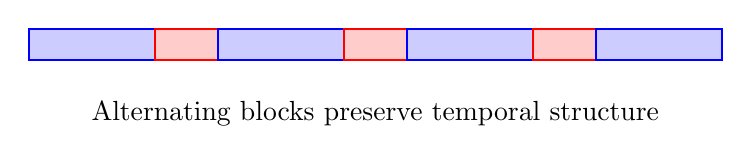
\begin{tikzpicture}[scale=0.8]
    % Blocks
    \draw[thick, blue, fill=blue!20] (0,1) rectangle (2,1.5);
    \draw[thick, red, fill=red!20] (2,1) rectangle (3,1.5);
    \draw[thick, blue, fill=blue!20] (3,1) rectangle (5,1.5);
    \draw[thick, red, fill=red!20] (5,1) rectangle (6,1.5);
    \draw[thick, blue, fill=blue!20] (6,1) rectangle (8,1.5);
    \draw[thick, red, fill=red!20] (8,1) rectangle (9,1.5);
    \draw[thick, blue, fill=blue!20] (9,1) rectangle (11,1.5);
    
    \node[below] at (5.5,0.5) {Alternating blocks preserve temporal structure};
\end{tikzpicture}
\end{center}

\section{Nested Cross-Validation}

When doing both model selection and performance estimation, we need nested CV to avoid optimistic bias.

\subsection{The Problem with Simple CV}

If you use the same CV folds for both hyperparameter tuning and final evaluation, you're indirectly using test data for training!

\subsection{Nested CV Solution}

\textbf{Two loops}:
\begin{itemize}
    \item \textbf{Outer loop}: Performance estimation (5-10 folds)
    \item \textbf{Inner loop}: Hyperparameter tuning (3-5 folds)
\end{itemize}

\begin{center}
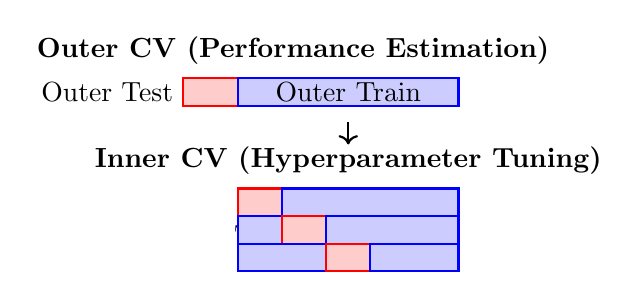
\begin{tikzpicture}[scale=0.7]
    % Outer CV
    \node at (2,4.5) {\textbf{Outer CV (Performance Estimation)}};
    
    % Outer fold visualization
    \draw[thick, red, fill=red!20] (0,3.5) rectangle (1,4);
    \draw[thick, blue, fill=blue!20] (1,3.5) rectangle (5,4);
    \node[left] at (0,3.75) {Outer Test};
    \node at (3,3.75) {Outer Train};
    
    % Arrow down
    \draw[->, thick] (3,3.2) -- (3,2.8);
    
    % Inner CV
    \node at (3,2.5) {\textbf{Inner CV (Hyperparameter Tuning)}};
    
    % Inner folds
    \draw[thick, red, fill=red!20] (1,1.5) rectangle (1.8,2);
    \draw[thick, blue, fill=blue!20] (1.8,1.5) rectangle (5,2);
    \node[below] at (1.4,1.5) {Test};
    \node[below] at (3.4,1.5) {Train};
    
    \draw[thick, blue, fill=blue!20] (1,1) rectangle (1.8,1.5);
    \draw[thick, red, fill=red!20] (1.8,1) rectangle (2.6,1.5);
    \draw[thick, blue, fill=blue!20] (2.6,1) rectangle (5,1.5);
    
    \draw[thick, blue, fill=blue!20] (1,0.5) rectangle (2.6,1);
    \draw[thick, red, fill=red!20] (2.6,0.5) rectangle (3.4,1);
    \draw[thick, blue, fill=blue!20] (3.4,0.5) rectangle (5,1);
\end{tikzpicture}
\end{center}

\textbf{Algorithm}:
\begin{enumerate}
    \item Split data into outer folds
    \item For each outer fold:
    \begin{itemize}
        \item Use outer training set for inner CV
        \item Find best hyperparameters via inner CV
        \item Train final model with best hyperparameters
        \item Evaluate on outer test fold
    \end{itemize}
    \item Average outer fold scores for unbiased estimate
\end{enumerate}

\section{Common Pitfalls and Best Practices}

\subsection{Data Leakage}

\textbf{Preprocessing before splitting}: WRONG!
\begin{verbatim}
# Wrong way
data_normalized = normalize(data)
train, test = split(data_normalized)
\end{verbatim}

\textbf{Preprocessing within each fold}: RIGHT!
\begin{verbatim}
# Right way
for train, test in cv_splits:
    train_normalized = normalize(train)
    test_normalized = normalize_with_train_params(test, train)
\end{verbatim}

\begin{tcolorbox}[colback=red!5!white,colframe=red!75!black,title=Example \stepcounter{example}\#\theexample: The Leakage Problem]

\textbf{Scenario}: You're predicting house prices and normalize features using mean/std of entire dataset before CV.

\textbf{Problem}: Test fold statistics influence the normalization of training folds!

\textbf{Impact}: Optimistically biased performance estimates. In extreme cases, can lead to 10-20\% overestimation of accuracy.

\textbf{Solution}: Compute normalization parameters only on training folds, apply to test fold.
\end{tcolorbox}

\subsection{Choosing k}

\textbf{Common choices}:
\begin{itemize}
    \item $k = 5$: Good balance of bias and variance
    \item $k = 10$: More stable, higher computational cost
    \item $k = n$ (LOOCV): Low bias, high variance, expensive
\end{itemize}

\textbf{Bias-variance trade-off}:
\begin{itemize}
    \item \textbf{Small k}: Lower variance (more training data), higher bias
    \item \textbf{Large k}: Higher variance (less training data), lower bias
\end{itemize}

\subsection{Statistical Significance}

\textbf{Comparing models}: Use paired t-test on CV fold scores
$$t = \frac{\bar{d}}{\text{SE}(\bar{d})} = \frac{\bar{d}}{s_d / \sqrt{k}}$$

where $d_i$ is the difference in performance between two models on fold $i$.

\textbf{Confidence intervals}:
$$\mu \pm t_{\alpha/2, k-1} \times \frac{s}{\sqrt{k}}$$

\section{Advanced Topics}

\subsection{Repeated Cross-Validation}

Repeat CV multiple times with different random splits to get more stable estimates:

$$\text{Repeated CV} = \frac{1}{r} \sum_{j=1}^r \text{CV}_j$$

where $r$ is the number of repetitions. Reduces variance but increases computational cost.

\subsection{Bootstrap Methods}

Alternative to CV using resampling with replacement:

\textbf{Bootstrap .632 estimator}:
$$\text{Err}_{.632} = 0.368 \times \text{Err}_{\text{train}} + 0.632 \times \text{Err}_{\text{boot}}$$

Addresses optimistic bias of bootstrap by combining training error and out-of-bag error.

\subsection{Learning Curves}

Use CV to understand how performance scales with training set size:

\begin{center}
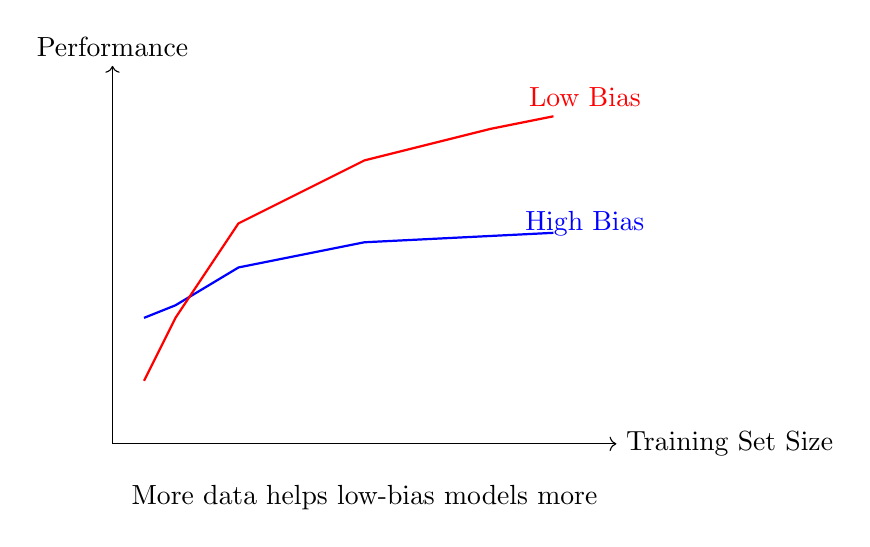
\begin{tikzpicture}[scale=0.8]
    \draw[->] (0,0) -- (8,0) node[right] {Training Set Size};
    \draw[->] (0,0) -- (0,6) node[above] {Performance};
    
    % High bias model
    \draw[thick, blue] (0.5,2) -- (1,2.2) -- (2,2.8) -- (4,3.2) -- (6,3.3) -- (7,3.35);
    \node[blue] at (7.5,3.5) {High Bias};
    
    % Low bias model  
    \draw[thick, red] (0.5,1) -- (1,2) -- (2,3.5) -- (4,4.5) -- (6,5) -- (7,5.2);
    \node[red] at (7.5,5.5) {Low Bias};
    
    \node[below] at (4,-0.5) {More data helps low-bias models more};
\end{tikzpicture}
\end{center}

\section{Implementation Guidelines}

\subsection{Computational Considerations}

\textbf{Time complexity}: $O(k \times T)$ where $T$ is model training time
\textbf{Space complexity}: Usually $O(1)$ if models aren't stored

\textbf{Optimization strategies}:
\begin{itemize}
    \item Parallel fold evaluation
    \item Early stopping for clearly bad hyperparameters
    \item Warm starts for iterative algorithms
    \item Cached preprocessing
\end{itemize}

\subsection{Practical Workflow}

\begin{enumerate}
    \item \textbf{Choose CV strategy} based on data characteristics
    \item \textbf{Set up preprocessing pipeline} that fits within folds
    \item \textbf{Define hyperparameter grid} for tuning
    \item \textbf{Run nested CV} if doing model selection
    \item \textbf{Analyze results} with confidence intervals
    \item \textbf{Validate on final holdout} set
\end{enumerate}

\section{Practice Problems}

\subsection{Basic Problems}

\begin{tcolorbox}[colback=gray!5!white,colframe=gray!75!black,title=Problem \stepcounter{exercise}\#\theexercise: CV Score Calculation]

You perform 5-fold CV on a binary classification problem and get these confusion matrices:

Fold 1: TP=18, FN=2, FP=3, TN=17\\
Fold 2: TP=16, FN=4, FP=2, TN=18\\
Fold 3: TP=19, FN=1, FP=4, TN=16\\
Fold 4: TP=17, FN=3, FP=1, TN=19\\
Fold 5: TP=15, FN=5, FP=2, TN=18

Calculate the mean accuracy and 95\% confidence interval.

\textbf{Solution}:
Fold accuracies: [0.875, 0.85, 0.875, 0.925, 0.825]
Mean = 0.87, Std = 0.0374
95\% CI: $0.87 \pm 1.96 \times 0.0374 = [0.797, 0.943]$
\end{tcolorbox}

\begin{tcolorbox}[colback=gray!5!white,colframe=gray!75!black,title=Problem \stepcounter{exercise}\#\theexercise: Choosing the Right CV]

For each scenario, choose the most appropriate CV method:

\textbf{a)} Predicting daily stock prices using past 5 years of data\\
\textbf{b)} Classifying medical images with 10,000 samples from 100 patients\\
\textbf{c)} Binary classification with 95\% negative, 5\% positive examples\\
\textbf{d)} Small dataset with 50 samples for hyperparameter tuning

\textbf{Solutions}:
a) Time series CV / Forward chaining
b) Group CV (group by patient)
c) Stratified CV
d) LOOCV or repeated CV
\end{tcolorbox}

\subsection{Advanced Problems}

\begin{tcolorbox}[colback=gray!5!white,colframe=gray!75!black,title=Problem \stepcounter{exercise}\#\theexercise: Nested CV Analysis]

You have 1000 samples and want to:
1. Compare 3 algorithms
2. Tune hyperparameters for each
3. Get unbiased performance estimate

Design a nested CV strategy with computational budget considerations.

\textbf{Solution}:
- Outer CV: 5-fold for final comparison
- Inner CV: 3-fold for hyperparameter tuning
- Total model fits: $5 \times 3 \times 3 \times H$ where $H$ is hyperparameter combinations
- Use parallel processing and early stopping to manage computational cost
- Report performance as mean $\pm$ std across outer folds
\end{tcolorbox}

\section{Summary and Guidelines}

\subsection{Key Takeaways}

\begin{enumerate}
    \item \textbf{Choose CV method based on data structure}: Regular k-fold for i.i.d. data, stratified for imbalanced classes, time series CV for temporal data, group CV for clustered data
    
    \item \textbf{Avoid data leakage}: Always preprocess within CV folds, never on the entire dataset
    
    \item \textbf{Use nested CV for model selection}: Prevents optimistic bias when tuning hyperparameters
    
    \item \textbf{Report confidence intervals}: Mean performance alone is insufficient; include variability estimates
    
    \item \textbf{Validate final model}: Use a separate holdout set for final validation after all CV-based decisions
\end{enumerate}

\subsection{Decision Tree for CV Method Selection}

\begin{center}
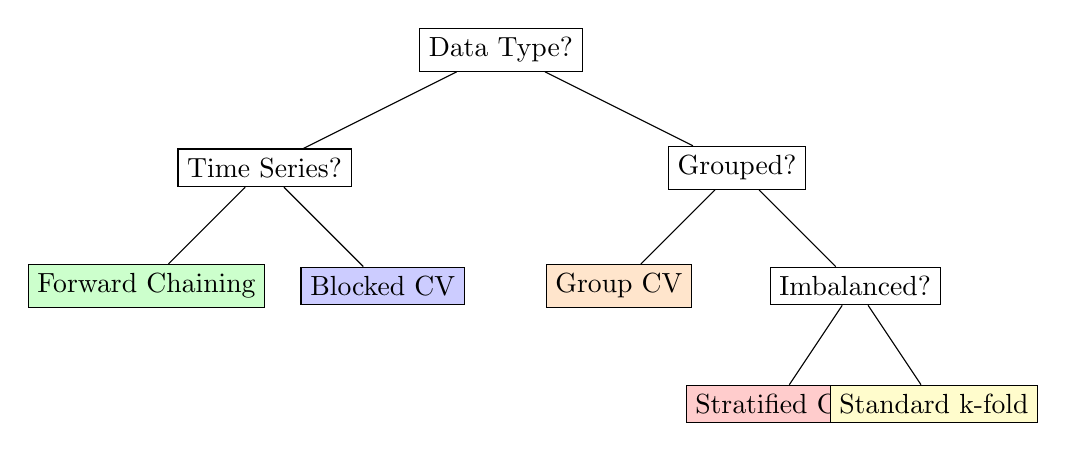
\begin{tikzpicture}[
  level distance=1.5cm,
  level 1/.style={sibling distance=6cm},
  level 2/.style={sibling distance=3cm},
  level 3/.style={sibling distance=2cm}
]
\node [rectangle, draw] {Data Type?}
  child {node [rectangle, draw] {Time Series?}
    child {node [rectangle, draw, fill=green!20] {Forward Chaining}}
    child {node [rectangle, draw, fill=blue!20] {Blocked CV}}
  }
  child {node [rectangle, draw] {Grouped?}
    child {node [rectangle, draw, fill=orange!20] {Group CV}}
    child {node [rectangle, draw] {Imbalanced?}
      child {node [rectangle, draw, fill=red!20] {Stratified CV}}
      child {node [rectangle, draw, fill=yellow!20] {Standard k-fold}}
    }
  };
\end{tikzpicture}
\end{center}

\subsection{Best Practices Checklist}

\begin{itemize}
    \item[$\square$] Choose appropriate CV method for your data structure
    \item[$\square$] Use stratification for classification problems
    \item[$\square$] Implement preprocessing within CV folds
    \item[$\square$] Use nested CV for hyperparameter tuning
    \item[$\square$] Report mean $\pm$ standard deviation/confidence interval
    \item[$\square$] Check for statistical significance when comparing models
    \item[$\square$] Reserve final holdout set for ultimate validation
    \item[$\square$] Consider computational budget when choosing $k$
\end{itemize}

\section{Further Reading}

\begin{itemize}
    \item \textbf{Comprehensive Review}: Arlot \& Celisse "A survey of cross-validation procedures for model selection" (2010)
    \item \textbf{Time Series CV}: Hyndman \& Athanasopoulos "Forecasting: Principles and Practice"
    \item \textbf{Statistical Analysis}: Dietterich "Approximate Statistical Tests for Comparing Supervised Classification Learning Algorithms" (1998)
    \item \textbf{Practical Guide}: Kuhn \& Johnson "Applied Predictive Modeling"
    \item \textbf{Modern Implementation}: scikit-learn cross-validation documentation
\end{itemize}

\end{document}